\section{Исследовательский раздел}
В этом разделе будет проведено исследование эффективности разработанного программного обеспечения.
Будет исследована зависимость метрики PSNR от выбранного порога применения медианного фильтра.
Будет проведено сравнение результатов работы реализованного метода с результатами, полученными с помощью известных аналогов.
Будет произведена оценка разработанного программного комплекса.

\subsection{Исследование зависимости метрики PSNR от порога применения}
В описании алгоритма было указано, что применение к исходному изображению медианного фильтра зависит от выбранного порога, который требовалось практически.

Для исследования зависимости было провести тестирование метода на трех различных значениях фильтра: 5\% загрязненности, 15\% загрязненности и 25\% загрязненности изначального изображения, и затем сравнить поведение метрик в зависимости от процента шума.

Требуется определить, при каком пороге значение метрик будет расти с началом применения медианного фильтра и восстанавливающей нейронной сети.
В дальнейшем предполагается использование выбранного порога для сравнения с другими методами.

\newpage
Результаты сравнения с аналогами представлен на графике \ref{res::comp}:
\FloatBarrier
\begin{figure}[h]	
	\begin{center}
		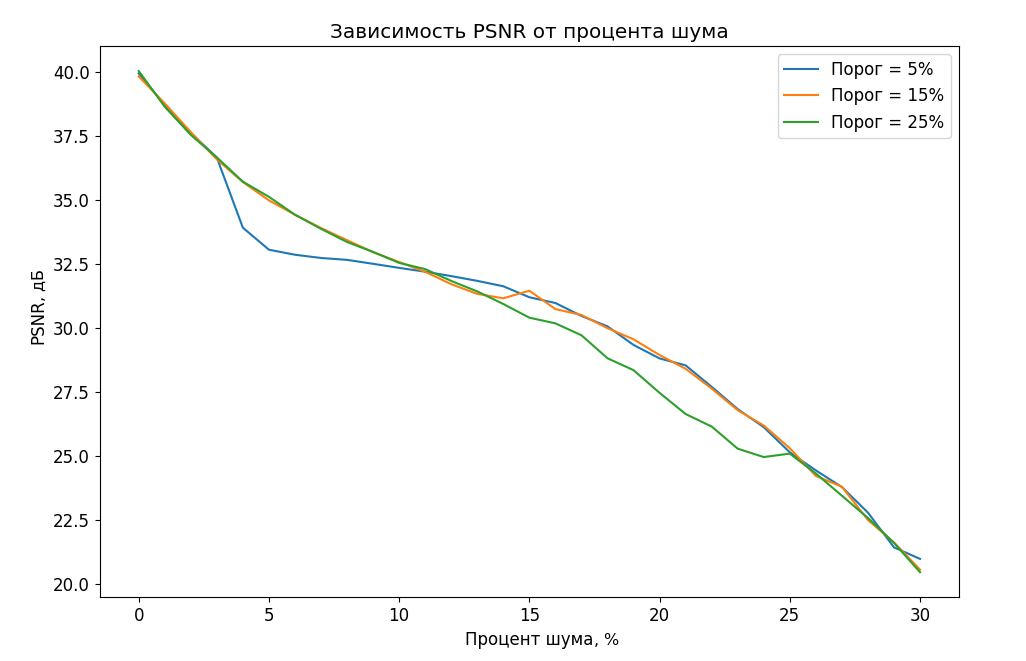
\includegraphics[width=\linewidth]{inc/png/median1.png}
	\end{center}
	\captionsetup{justification=centering}
	\caption{Сравнение эффективности метода в зависимости от порога}
	\label{res::comp}
\end{figure}
\FloatBarrier

Выяснилось, что наилучшие результаты показал алгоритм, применяющий фильтр в случае 15\% уровня загрязненности патча.
При 5\% порога падение оказывается слишком резким, при 25\% уровне порога значение PSNR снижается быстрее, чем при 15\% пороге.

\subsection{Сравнение реализованного метода с аналогами}
В качестве аналогов, которые рассматривались для сравнения с реализованным методов, были выбраны:
\begin{enumerate}
	\item Медианный фильтр.
	\item Билатеральный фильтр.
	\item RIDNET.
\end{enumerate}

Этот выбор связан с тем, что фильтры являются самыми распространенными методами борьбы с импульсными шумами, а разработанный алгоритм позволяет устранить недостатки метода RIDNET.

Результаты сравнения с аналогами представлен на графике \ref{res::conp}:
\FloatBarrier
\begin{figure}[h]	
	\begin{center}
		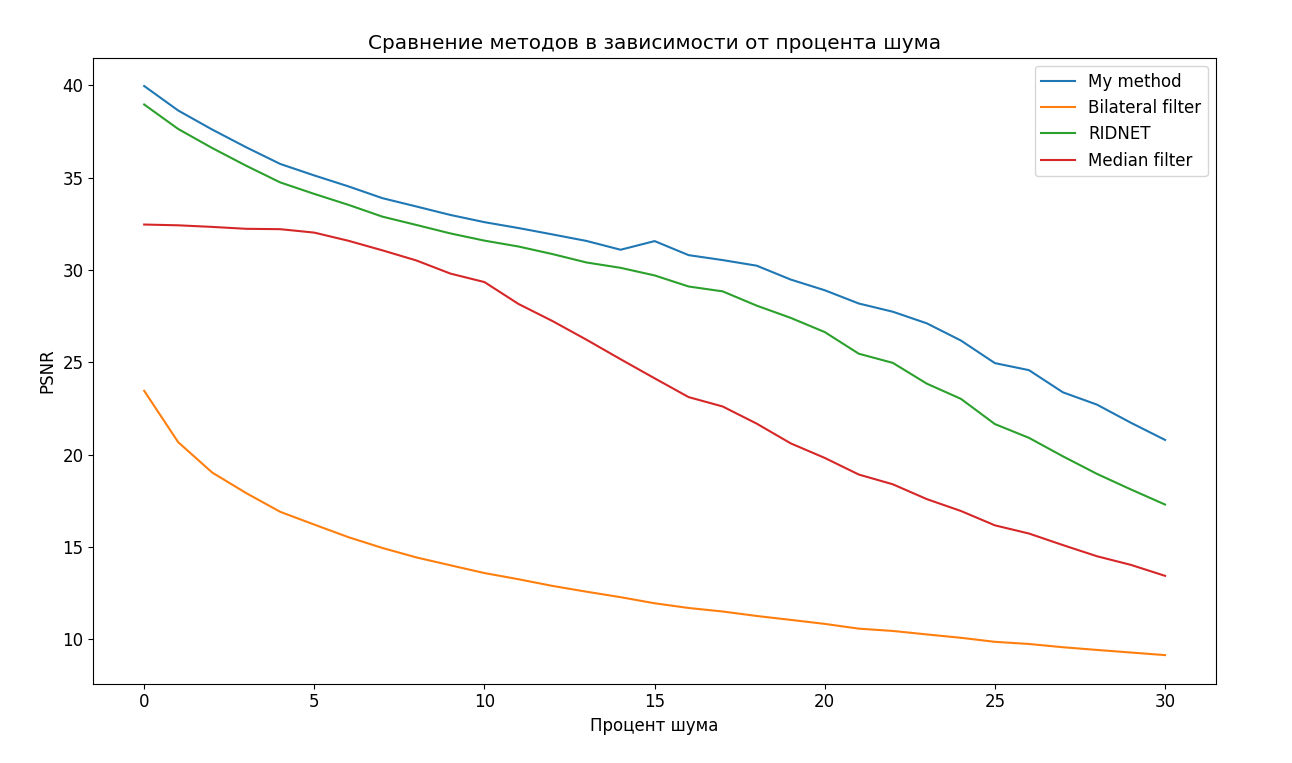
\includegraphics[width=\linewidth]{inc/png/result1.png}
	\end{center}
	\captionsetup{justification=centering}
	\caption{Сравнение методов в зависимости от типа шума}
	\label{res::conp}
\end{figure}
\FloatBarrier

Из графика можно сделать следующие выводы:
\begin{itemize}
	\item все методы имеют тенденцию к снижению метрики PSNR с увеличением количества шума на изображении;
	\item реализованный в работе метод является самым эффективным алгоритмом среди всех перечисленных;
	\item разработанный метод дает в результате более высокие метрики, чем исходный RIDNET, особенно на степени загрязненности изображения 15\% и больше.
\end{itemize}

Разработанный алгоритм позволил лучше справляться с изображениями, которые значительно загрязнены шумами.

\subsection{Оценка разработанного программного комплекса}
У разработанного программного комплекса можно выделить следующие \textbf{преимущества}:
\begin{enumerate}
	\item Универсальность. Алгоритм работает с любым размером изображений, превышающих минимальный размер -- 40 х 40 пикселей.
	\item Алгоритм не требует от пользователя предварительного ввода процента шума.
	\item Алгоритм позволяет работать с любым типом импульсного шума: шума соли или шума перца.
	\item По сравнению с известными аналогами, алгоритм показывает более высокие результаты.
\end{enumerate}

Также можно выделить некоторые \textbf{недостатки} метода:
\begin{enumerate}
	\item Изображение на выходе получается слегка размытым, что является следствием применения медианного фильтра.
	\item Медианный фильтр влияет на все пиксели изображения, в то время как можно его применять лишь к пикселям, идентифицированным как шум.
	\item Не поддерживаются другие форматы, кроме JPG.
\end{enumerate}

\subsection*{Выводы}
Было проведено сравнение результатов работы реализованного метода с результатами, полученными с помощью известных аналогов.
Выяснилось, что алгоритм показывает лучшие показатели метрик по сравнению с ранее рассмотренными аналогами.
По результатам исследования эффективности ПО выяснилось, что оптимальный порог для применения медианного фильтра -- 15\% уровня загрязненности патча.
Была произведена оценка разработанного программного комплекса, где были выделены основные достоинства и недостатки ПО.